Recently, I was working on the project of ai gym trainer. So what you do is basically, record your vedio or turn on your camera for live rep counting. So follow is the idea:

The problem statement is simple, given a video, I have to count the number of reps user has performed and also check if the form of the user is correct or not. I have to do this in real time too, since I want to support video to from live vedio feed.

\textbf{Mediapipe}

I discovered this library, which is developed and maintained by Google. I used it to extract. To discuss on some of the core functionalities of mediapipe library, below image describes number of features that this library has.

\begin{figure}[H]
    \centering
    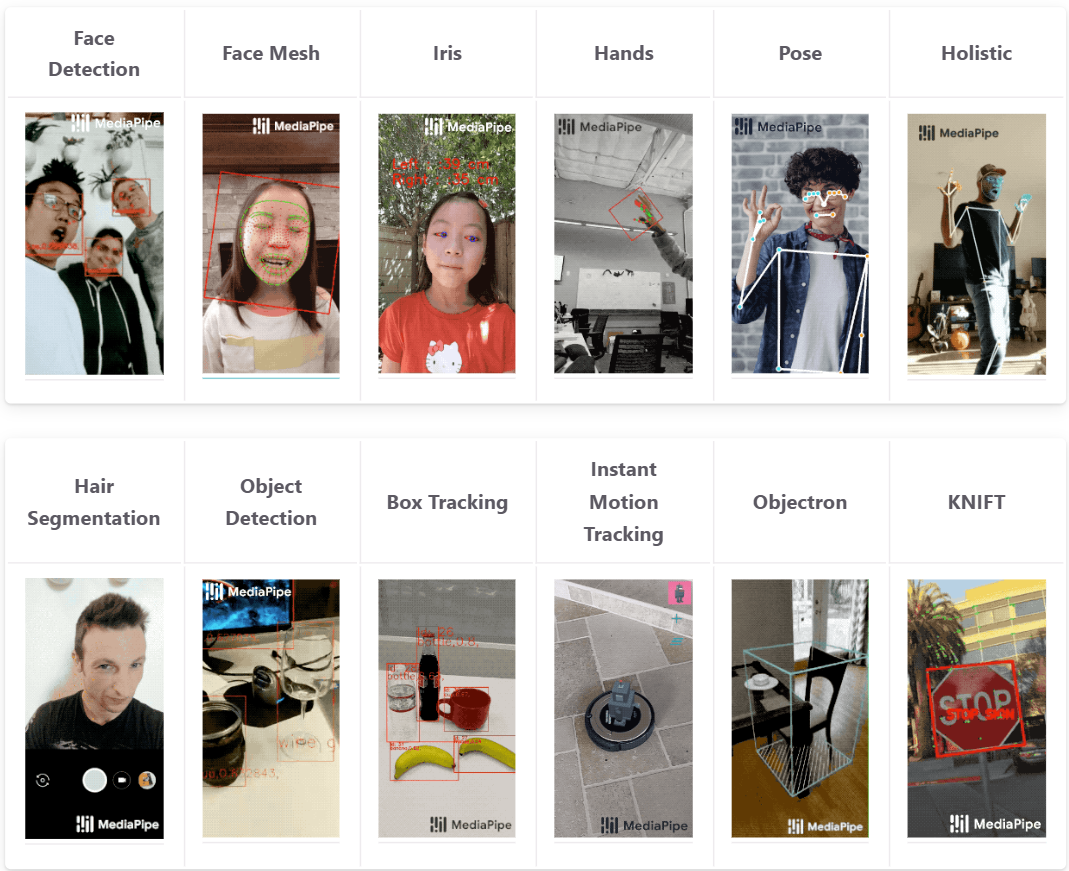
\includegraphics[width=1.06\textwidth]{res/Mediapipe.png}
    \caption{Mediapipe features}
    \label{fig:2_mediapipe}
\end{figure}


\textbf{mediapipe}

I used it to extract skeleton of the human body currently in frame. This is a pose estimation problem


\begin{figure}[H]
    \centering
    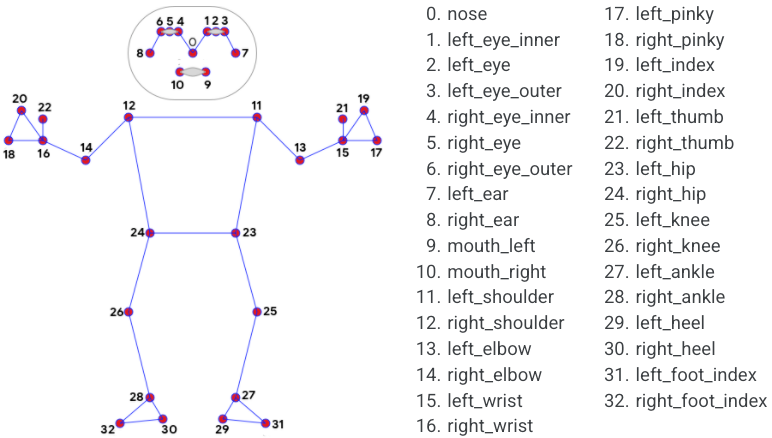
\includegraphics[width=1.06\textwidth]{res/pose_tracking_full_body_landmarks.png}
    \caption{Pose tracking full body landmarks}
    \label{fig:2_mpose_landmarks}
\end{figure}

I then used the extracted skeleton to extract the angles of the joints. I used these angles to figure if the angles cross certain threshold to count the rep. I also used the angles to figure out if the form of the person is correct or not.

I haved added a screenshot of working of that project.

\begin{figure}[H]
    \centering
    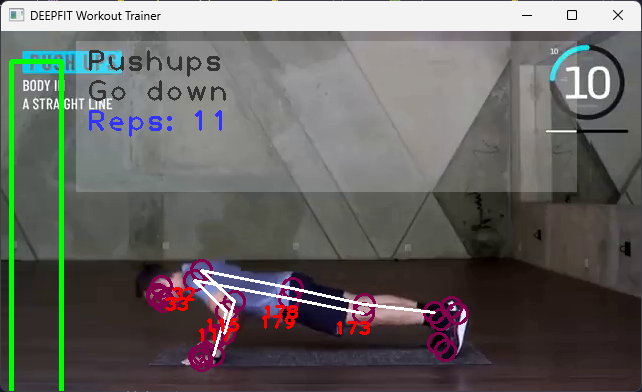
\includegraphics[width=.8\textwidth]{res/deepfit.png}
    \caption{AI gym trainer app}
    \label{fig:2_deepfit}
\end{figure}